\subsection{Wyniki - krzywe dyspersji}
\label{sec:53}

Rysunek \ref{fig:wykres4} przedstawia krzywe dyspersji otrzymane z wykorzystaniem elementów czworościennych, a rysunek \ref{fig:wykres8} krzywe otrzymane z wykorzystaniem elementów sześciennych.

\begin{figure}[h]
\centering
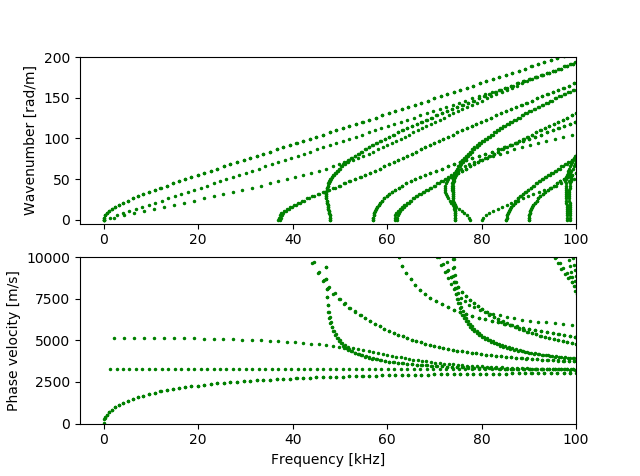
\includegraphics[width=14cm]{Zdjecia/5/wykres4}
\caption{Krzywe dyspersji otrzymane z wykorzystaniem elementów czworościennych dla stalowego pręta o promieniu 25mm.
Pozostałe parametry symulacji to num\_of\_circles = 8 oraz num\_of\_points\_at\_c1 = 8}
\label{fig:wykres4}
\end{figure}

\begin{figure}[h]
\centering
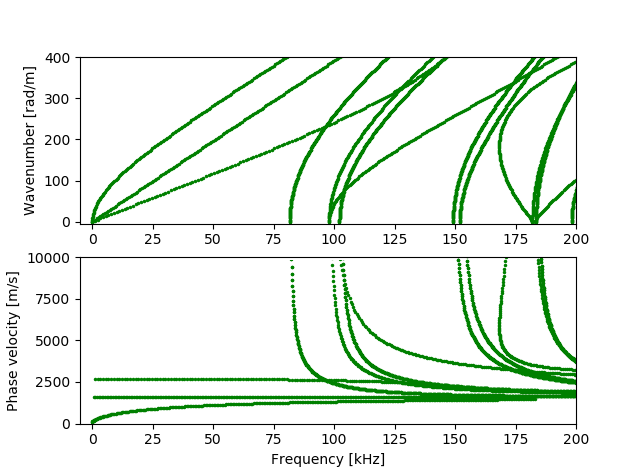
\includegraphics[width=14cm]{Zdjecia/5/wykres8}
\caption{Krzywe dyspersji otrzymane z wykorzystaniem elementów sześciennych dla stalowego pręta o promieniu 25mm.
Pozostałe parametry symulacji to firstCircle = 16, addNodes = 0, circles = 2}
\label{fig:wykres8}
\end{figure}


Wyniki różnią się do siebie częstotliwościami, w których pojawiają się kolejne postaci fali. Biorąc pod uwagę spodziewane wyniki, symulacja z wykorzystaniem elementów sześciennych wprowadza błąd na nieznanym etapie. Prędkości fali różnią się mocno od oczekiwanych.

W przypadku symulacji z elementami czworościennymi wyniki zbiegają do oczekiwanych wraz z zagęszczaniem siatki elementów. Przedstawia to rysunk \ref{fig:porownanie}. Widać na nim, że różnica pomiędzy wynikami z najrzadszą siatką, a wynikami ze średnią siatką, jest większa niż pomiędzy tą drugą, a siatką najgęstszą.  Na tej podstawie można wywnioskować, że obliczenia przebiegają poprawnie.

\begin{figure}[h]
\centering
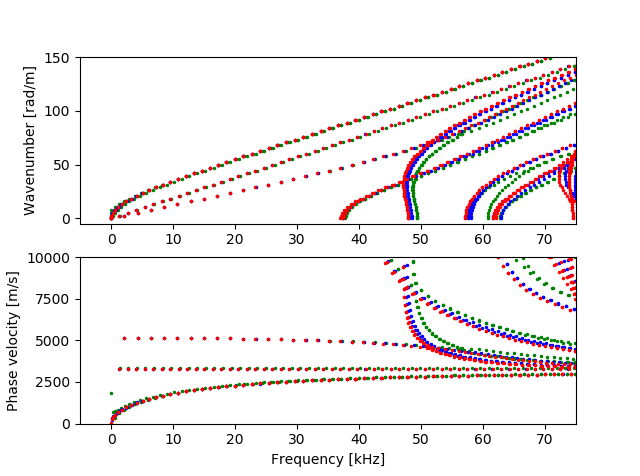
\includegraphics[width=14cm]{Zdjecia/5/porownanie}
\caption{Porównanie wyników z różną gęstością siatki. Kolor zielony - najrzadsza, niebieski - średnia, czerwony - najgęstsza}
\label{fig:porownanie}
\end{figure}